\section{Technical fundamentals}

This section will explain the technical fundamentals which are necessary to understand the full bachelor thesis.

\subsection{The Scapy library}

%UDS stack
\begin{wrapfigure}{r}{0.15\textwidth}
    %
\includegraphics[width=0.1\textwidth]{scapy_logo}
    \raisebox{0pt}[\dimexpr\height-1.5\baselineskip\relax]{
\includegraphics[width=0.15\textwidth]{scapy_logo}}
    %\label{fig:scapy-logo}
\end{wrapfigure}

Scapy \cite{scapy} is a Python program that enables the user to send, sniff and dissect and forge network packets. This capability allows construction of tools that can probe, scan or attack networks.

It can be imagined similar to Wireshark, except that its usage happens in the terminal and not only allows reading network packets, but also crafting and sending them. It can also be used as a library by importing the necessary classes and interfaces into the own Python program. Scapy supports Python 3 and additionally Python 2, even though its support has ended on 1st of January 2020. The following quote from a maintainer explains the reason behind that \cite{scapy-py2}:

\begin{displayquote}
    Scapy is a tool that can be used in a very large number of situations. Often, you don't get to choose the Python interpreter you have when you run Scapy. So, [...] we need to keep supporting Python 2.7 as long as we can.
\end{displayquote}

Understanding Scapy will be important for the later implementation in this work, since the UDS Scanner to be modified in this work is built within Scapy.

One of the core classes in Scapy is the \textbf{Packet} class. All definitions of network packet layers, such as Ethernet, IP, TCP, CAN, UDS and so on, are defined in a class inheriting from that class.

The well-known and simple UDP protocol \cite{udp} serves as an illustrative example.

For this it will be shown how the UDP header, shown in \autoref{fig:uds_header} is translated to such a Scapy class.

%UDP header
\begin{figure}[h]
    \centering
    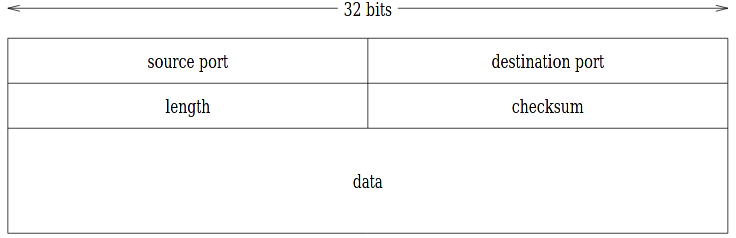
\includegraphics[width=0.7\textwidth]{udp_header}
    \caption{UDP header format \cite{udp_header}}
    \label{fig:uds_header}
\end{figure}

The UDP header format contains four fields and the data field. These four fields are translated literally into the Scapy class \textbf{UDP}. The data field is not part of it because Scapy uses an explicit operator to append data to the header information. This is shown later.

The following code snippet shows the explained class in the Scapy library.

\begin{samepage}
\begin{minted}{python}
class UDP(Packet):
   fields_desc = [ShortEnumField("sport", 53, UDP_SERVICES),
                  ShortEnumField("dport", 53, UDP_SERVICES),
                  ShortField("len", None),
                  XShortField("chksum", None)]
\end{minted}
\end{samepage}

As in common programmer language, \textbf{short} specifies 16 bits. Since the UDP header only contains 16 bits fields, the Scapy definition only includes \textbf{short} fields. The first parameter of a field is always the name of this field. \textbf{sport} stands for source port, and \textbf{dport} for destination port.
The next parameter sets the default value for this field. This is defined by the Scapy programmers in all conscience and not by the official UDP standard. \textbf{53} specifies the DNS protocol.
\textbf{EnumField}s also contain a third argument. This is a simple dictionary mapping from machine-readable values to human-readable texts. For example, part of the \textbf{UDP\_SERVICES} dictionary is: \mintinline{python}{{53: "domain", 80: "www_http"}}
The difference of ShortField and XShortField is only in the representation. The value of the XShortField will be displayed as a hex value and the ShortField as a decimal value.

The following snippets shows some examples of how to instantiate an object of the UDP class and also demonstrates how to append data to the headers with the “/” operator.

\begin{samepage}
\begin{minted}{python}
packet = UDP(dport=80) # is equivalent to:
packet = UDP(dport="www_http")

# Append 0x00 as data
packet = UDP(dport=80) / Raw(b'\x00')
\end{minted}
\end{samepage}

Now it shall be explained, how to actually send a packet and receive a response. For this, a socket is required. Scapy provides many kinds of sockets for different use cases. For example the \textbf{L2Socket} and the \textbf{L3PacketSocket}. The difference between them is that L2Socket expects a packet object containing all information starting from Ethernet (Layer 2), while L3PacketSocket expected a packet object only containing all information starting from IP (layer 3). The following code snippet uses the L2Socket for full coverage of the whole packet stack and explains how sending and receiving of a packet works (Note: Root privileges might be necessary for this to work):

\begin{samepage}
\begin{minted}{python}
# import necessary classes
from scapy.arch.linux import L2Socket
# Create a layer 2 socket specifing the interface name
socket = L2Socket("eth0")
# Create a packet covering layer 2 to 7, targeting the Google server
# This packet starts a TCP handshake, thus the SYN flag is exclusively set
# Set destination port to HTTP and a high source port
packet = Ether() / IP(dst="142.250.185.163") / TCP(flags="S", dport=80, sport=60123)
# sr1 stands for: send receive one
# it sends the given packet and returns the response
response = socket.sr1(packet)
# This displays the response in a human-friendly form
response.show()
\end{minted}
\end{samepage}

The .show() command gives the following output. It has been slightly edited to be more compact and some information has been replaced by placeholders for privacy reasons.

\begin{samepage}
\begin{minted}{text}
###[ Ethernet ]### 
  dst       = 12:34:45:67:89:ab
  src       = 2c:3a:fd:af:64:e0
  type      = IPv4
###[ IP ]### 
     version   = 4
     src       = 142.250.185.163
     dst       = 123.123.123.123
###[ TCP ]### 
        sport     = www_http
        dport     = 60123
        flags     = SA
\end{minted}
\end{samepage}

The SYN and ACK flags are set now as expected for the TCP handshake. Furthermore, the dport of the response is the sport of the request.

The UDS Scanner later described in this work is mainly, but not exclusively, used with the ISOTP protocol. It is the transport protocol for the CAN bus (Controller Area Network). Thus, it will be explained here as well.

There are two ISOTP socket implementations in Scapy. A software and a native implementation. The native implementation is only usable for Linux but the preferred one, since it uses the socket interface of Linux and brings all its advantages. Until including Linux kernel 5.9, the corresponding ISOTP module for Linux had to be installed separately \cite{isotp-module}. Since Linux kernel 5.10, it is part of the Linux mainline kernel \cite{isotp-commit}.

To create a virtual CAN interface, one line in a shell is sufficient:
\begin{samepage}
\begin{minted}{text}
sudo ip link add vcan0 type vcan
\end{minted}
\end{samepage}

An ISOTP socket contains a source and destination identifier. The source identifier is the identifier the outgoing CAN packets will contain. The destination identifier is the identifier expected for incoming packets.

The usage of the native implementation is illustrated in the following code snippet:

\begin{samepage}
\begin{minted}{python}
from scapy.contrib.isotp import ISOTPNativeSocket
socket = ISOTPNativeSocket("vcan0", sid=0x123, did=0x456)
packet = Raw(b"\x01\x02")
socket.send(packet)
\end{minted}
\end{samepage}


\subsection{The UDS protocol}

UDS stands for \emph{Unified diagnostic services} and is an application protocol defined in ISO 14229 \cite{iso14229}. This protocol contains information about the structure of diagnostic request and response packets sent over an arbitrary data link.

%UDS stack
\begin{figure}[h]
    \centering
    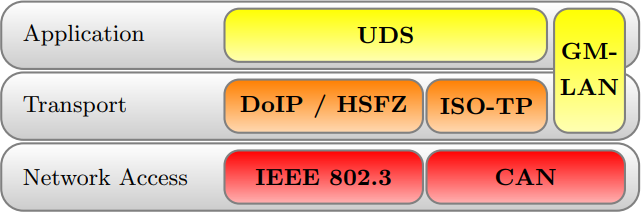
\includegraphics[width=0.7\textwidth]{uds-stack}
    \caption{The most common protocol stack for UDS \cite{Weiss2020}}
    \label{fig:uds-stack}
\end{figure}

As shown in \autoref{fig:uds-stack}, the most common data links for the UDS protocol are the Ethernet and the CAN protocol. Others can and are used as well, explicitly stated in the UDS standard are FlexRay, K-Line and LIN.

The UDS protocol defines various services with different purposes. For example the DiagnosticSessionControl service is used to enable different diagnostic sessions in the ECU. Its identifier is the number 0x10. All packets requesting this service specify this value as the first byte. The response identifiers are defined as 0x40 added to the request identifier. Thus, for the DiagnosticSessionControl the positive response identifier is 0x10 + 0x40 = 0x50. A negative response always has the identifier 0x7f. This service is able to change the state of the ECU. The ReadDataByIdentifier service is not able to change the state, yet it is very important. Data records in the ECU are stored with an identifier as the key. This service allows to read these values from an external device. Since there can be data stored, which is not meant to be read by everybody, there is another service called SecurityAccess, which allows to unlock these information for external devices. This mechanism is used for other services as well. The SecurityAccess uses the challenge–response authentication and follows the following sequence \cite{iso14229}:

\begin{samepage}
\begin{enumerate}
  \item client requests the “Seed”,
  \item server sends the “Seed”,
  \item client sends the “Key” (appropriate for the Seed received),
  \item server responds that the “Key” was valid and that it will unlock itself.
\end{enumerate}
\end{samepage}

Now the implementation in Scapy will be described.

\begin{samepage}
\begin{minted}{python}
class UDS(ISOTP):
    services = ObservableDict(
        {0x10: 'DiagnosticSessionControl',
         # [...]
         0x22: 'ReadDataByIdentifier',
         # [...]
         0x7f: 'NegativeResponse'})
    fields_desc = [
        XByteEnumField('service', 0, services)
    ]
\end{minted}
\end{samepage}

%TODO: Why inherting from ISOTP

The UDS class contains only the service field. Even though the whole UDS protocol is in layer 7, the Scapy implementation starts a new class whenever the subsequent fields depend on one field of the current layer. This is the case here, since the next fields depend on the value in the service field. The service specific fields are defined in their own classes, for example:

\begin{samepage}
\begin{minted}{python}
class UDS_DSC(Packet):
    diagnosticSessionTypes = ObservableDict({ ... })
    fields_desc = [
        ByteEnumField('diagnosticSessionType', 0,  diagnosticSessionTypes)
    ]
\end{minted}
\end{samepage}

A UDS packet enabling the extendedDiagnosticSession would be created with:

\begin{samepage}
\begin{minted}{python}
packet = UDS() / UDS_DSC(diagnosticSessionType="extendedDiagnosticSession")
\end{minted}
\end{samepage}


\subsection{The UDS Scanner}
